\section{Introduction}
\label{sec:introduction}

\begin{figure*}[t]
\centering
\subfigure{%
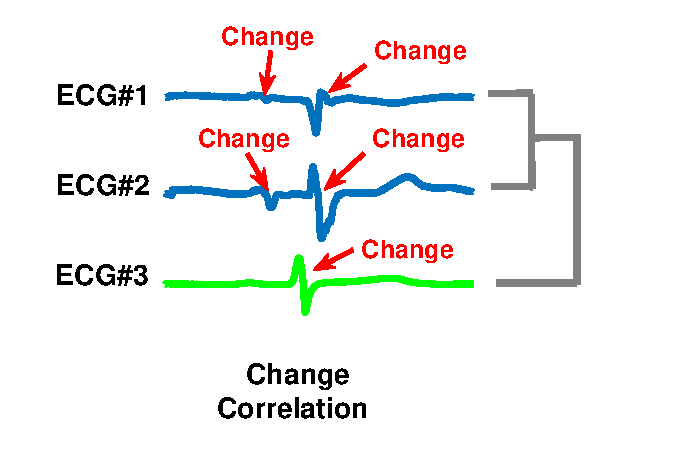
\includegraphics[width=0.30\textwidth]{ECGExChangeCorrelation.eps}
}\hspace{0.001em}
\subfigure{%
\includegraphics[width=0.30\textwidth]{ECGExDTW.eps}
}\hspace{0.001em}
\subfigure{%
\includegraphics[width=0.30\textwidth]{ECGExED.eps}
}\hspace{0.001em}
\caption{ Three ECG time series with two labels }
\label{fig:ecgexample}
\end{figure*}

\begin{figure}[t]
\centering
\includegraphics[width=0.45\textwidth]{HPCExample.pdf}
\caption{Three Thread time series}
\label{fig:hpcexample}
\end{figure}

The focus of this paper will be on the time series data. A time series is defined as a sequence of values $\{\}$ associated with timestamps $ $.

Time series mining is ubiquitous in data driven applications including robotics, medicine~\cite{}, speech~\cite{rabiner1993fundamentals}, object detection in vision~\cite{yang2002detecting, sonka2014image}, system failure diagnosis~\cite{luo2014correlating,sun2014querying}, ... more from the paper.  Due to its pervasive presence, time series mining have received significant attention in recent years. A common prerequisite for data mining algorithms, such as clustering, search, classification and regression, etc., is a measure of correlation (or similarity). Dynamic Time Warping (DTW) is widely accepted, and arguably the most popular, measure of similarity (or correlation) for time series data in general~\cite{}.

All existing measures over time series, including the popular DTW, relies on the notion that two time series $T_1$ and $T_2$ are similar, if there is a long enough similarly behaving subsequence common between them. This is a very reasonable notion which is also the desired nature of the similarity function in many applications.  However, there are plenty of real-world problems where the notions of similarity can be very different. Using existing similarity measures, such as DTW, for such problems often lead to misleading results. Despite their importance, there has been little previous work addressing those scenarios. To signify their importance, we provide two motivating real-world examples:

\textbf{Analysis of ECG (Electrocardiogram) data}

Electrocardiography \cite{holter1961new} (ECG or EKG*)
is the process of recording the electrical activity of the heart over a period of time using electrodes placed on a patient's body.
These electrodes detect the tiny electrical changes on the skin that arise from the heart muscle depolarizing during each heartbeat.
If two ECG often have tiny electrical changes at the same time, they can be regarded as correlated.\cite{marriott1988practical}.
By analyzing such data, one can find some useful information hidden behind the human body, thus to uncover some miracles of human body \cite{tilley1979essentials}.

%The first real-world example is ECG data\cite{holter1961new}. 
We take the ECG time series data from the UCR time series data Archive \cite{UCRArchive}, and the label is also provided by them.
We choose three time series from two different labels in that data set.
We illustrate this in Figure\ref{fig:ecgexample}, where we show the hierarchical clustering of these three time series under various measures. 
Top two red bold time series ($ECG\#1,ECG\#2$) are labeled as same class, and $ECG \#3$ is labeled as other class.

As we can see from Fig.\ref{fig:ecgexample}, Euclidean Distance and DTW Distance does poorly here. 
This is not surprising, since the ECG time series data have different change patterns (e.g. Increase-Decrease, Decrease-Increase, or a Sudden wave, etc.). These different change patterns can effect the performance of point to point similarity measures.
And the correlation of ECG time series is major focus on whether have tiny electrical change at the same time \cite{tilley1979essentials}.

{\bf \color{red} Clear mention, where the data comes from, what are the labels (categories whyc you colored blue and red). And what is the value of the pairwise similarity between those 3 examples with DTW, our measure and L2 distance. Argue why DTW and L2 does not lead to the required ordering. Explain in details and we will condense it later. Right now its handwavy and wont work.}


%correlation is a major research topic in data mining area.
%Such correlating techniques has been applied in many real world problems.
%For example, some researchers use time series correlation techniques to analysis the signal information for speech processing \cite{rabiner1993fundamentals}.
%Image processing researchers also use time series correlation techniques to deal with the image retrieval problems and object detection problems \cite{yang2002detecting, sonka2014image}.
%In the system diagnose area\cite{luo2014correlating,sun2014querying}, time series correlation techniques also widely used to mine the system behavior and diagnose system failures.
%Time series correlation techniques can also be used for analyzing bio-sequences (e.g DNA Sequence, etc \cite{mount2001bioinformatics} etc.

%In addition, real world time series are all high dimensional and large scale data, how to mining such huge amount of data set is also a challenge for us.

\textbf{Analysis of HPC Thread time series.}
High-performance computers (HPC) have become enormously complex. Today, the largest systems consist of more than tens of thousands of nodes. Nodes themselves are equipped with one or more multicore microprocessors\cite{adhianto2010hpctoolkit}. 
High-performance computer can generate over billions of threads during running.
And how to automatically analysis and monitoring the HPC is a major task for HPC researchers \cite{mccurdy2010memphis,tallent2009effective}.

%As a result, it is increasingly difficult for application developers writing complex scientific programs to attain a significant fraction of peak performance on modern microprocessor-based computer systems.

HPCToolkit\footnote{http://hpctoolkit.org/} can be used to generate the performance information of each thread from HPC. 
And each thread can be represented as a time series. The value of the time series denote the state of the thread.

%(Depend on which aspect of a thread to be represent, domain knowledge required) The thread change information (e.g. change from one state to another state) can directly reflect some important properties of different threads.

Fig. \ref{fig:hpcexample} shows a example of three thread time series data. Different colors means different state they are in. 
\textbf{Thread \#1}, and \textbf{Thread \#2} are in the same class, and \textbf{Thread \#3} is in the other class. The ground truth is provided by the HPCToolkit team\footnote{http://hpctoolkit.org/}.

The DTW distance between \textbf{Thread \#1}, and \textbf{Thread \#2} is $0.83$. While the DTW distance between \textbf{Thread \#2}, and \textbf{Thread \#3} is $0.31$. While the DTW distance between \textbf{Thread \#1}, and \textbf{Thread \#3} is $0.51$. 

The Euclidean distance between \textbf{Thread \#1}, and \textbf{Thread \#2} is $0.64$. While the DTW distance between \textbf{Thread \#2}, and \textbf{Thread \#3} is $0.53$. While the DTW distance between \textbf{Thread \#1}, and \textbf{Thread \#3} is $0.71$. 

The Change Correlation between \textbf{Thread \#1}, and \textbf{Thread \#2} is $1.00$. While the DTW distance between \textbf{Thread \#2}, and \textbf{Thread \#3} is $0.00$. 
While the DTW distance between \textbf{Thread \#1}, and \textbf{Thread \#3} is $0.00$. 

We can see that DTW and Euclidean distance can not perform well. Because \textbf{Thread \#1} and \textbf{Thread \#2} always have different states and DTW and Euclidean will regard these state difference as large distance.

On the other hand, change based correlation only consider the change information of the time series, and state difference between \textbf{Thread \#1}, and \textbf{Thread \#2} can not effect the correlation result.

As showed in above motivating examples, most of the existing time series similarity measures (e.g. L1-Distance, L2-Distance \cite{han2011data}, and DTW-Distance \cite{muller2007dynamic}, etc) or correlation measures (e.g. Pearson Correlation \cite{pearson1904mathematical}, Kendall rank correlation \cite{kendall1938new}, and Spearman's rank correlation \cite{pirie1988spearman}, etc.) can not deal with such heterogeneous properties of the time series: The change pattern differences between ECG time series and state different between thread time series.

The reason is: the correlation between heterogeneous time series is often associated with the change during a time period rather than a point-to-point corresponding relationship.
And the existing similarity and correlation measures only consider the point to point similarity or correlation between different time series.
%In this paper, we will introduce the related research in detail in Section \ref{sec:relatedwork}.
As a result, In order to deal with heterogeneity properties of time series with different patterns.
We proposed a change based correlation coefficient.
The intuition of this correlation is:


%However, in most real world problems, time series data often have different patterns (Heterogeneous time series). For example, in the area of system analysis area.
%Each performance counter can be regarded as a time series (e.g. CPU Usage, Memory Usage, etc.).
%Some of the time series may be a periodical time series, but others may be a linear or random patterns.
%However, heterogeneous time series may also be correlations between each other.
%So, how to calculate the correlation between heterogeneous time series data is a challenge.

\textit{If two time series often change at the same time, they may have correlation with each other.}

The detailed definition will be introduced in section \ref{sec:formulation}.
Our change based correlation method firstly extract the change information of the time series data, and then use the change information to calculate the correlation coefficient between the two time series.
We also use the hashing methods speed up the correlation calculation between time series, as well as searching and clustering.
So the computational cost of our coefficient is low, thus our method can also deal with the large scale property of the time series data.

The contribution of this paper is listed as follow:
\begin{enumerate}
\item Motivated by real applications, we investigate the correlation
problem as between heterogeneous time series (Time Series with different patterns).
To the best of our knowledge, this is the first attempt
to evaluate the correlation between time series with different patterns.

\item We proposed a correlation coefficient between heterogeneous time series, and
use hashing method to speed up the calculating of the coefficient between time series, as well as the clustering and nearest neighbors search tasks.

\item The experiments on Synthetic data show the effectiveness and efficiency of our method.
\end{enumerate}

The rest of the paper is organized as follows: In Section 2, we introduce the problem
statement and formulation. Our approach is proposed in Section 3. The Empirical evaluation is shown in Section 4. In Section 5, we introduce some
related works. Finally, we conclude our work in Section 6.



